
\chapter{Apache\textsuperscript{\footnotesize\texttrademark} Hadoop\textsuperscript{\footnotesize\textregistered}}
\section{¿Que es Apache Hadoop?}\label{sec:que_es_apache_hadoop}
\textbf{\textit{Apache Hadoop}}\index{Apache!Hadoop} es un software de procesamiento distribuido que permite almacenar 
y procesar grandes cantidades de datos sobre un \textit{cluster} (\autoref{sec:arquitectura_cluster})
 de máquinas (nodos del \textit{cluster}).
\textit{Hadoop} es un proyecto \textit{open source} de la \textit{Apache Software Foundation} creado inicialmente por
\textit{Doug Cuttin}, actualmente en desarrollo y mantenido por la comunidad de software libre.\\
El diseño de \textit{Hadoop} está enfocado a procesar los datos en el mismo nodo donde se encuentran,
llevando el código al dato y evitando así el cuello de botella resultante del tráfico de red
al transferir los datos. Este diseño es conocido como \textit{\textbf{data locality}\index{Data locality}}.
\textit{Hadoop} es escalable y tolerante a fallos, tanto en el almacenamiento de los datos como en el
procesamiento de estos. La tolerancia a fallos la gestiona mediante la replicación de los datos
en 3 copias (por defecto, configurable), cada una en un nodo distinto del cluster. 
De esta manera facilita así las oportunidades de \textit{data locality}, explicado anteriormente.

\noindent \textit{Apache Hadoop} se compone de dos partes fundamentales:
\begin{description}
  \item[HDFS](\textit{Hadoop Distributed File System})\index{Hadoop!HDFS}, es el software encargado de almacenar 
  y distribuir los datos a través de las máquinas del cluster. Es altamente escalable y tolerante a fallos.
  Cuando un archivo es subido al \textit{cluster}, este es dividido en bloques de $128 mb$ y replicado por
  3 sobre los nodos del \textit{cluster}.
  Su arquitectura esta basada en el tipo maestro-exclavo:
  \begin{itemize}
    \item \textit{NameNode}(Maestro) Contiene los metadatos de los archivos.
    \item \textit{NodeManager}(Exclavo) Contine los datos en sí del archivo.
  \end{itemize}

  \item[YARN] (\textit{Yet Another Resource Negotiator})\index{Hadoop!YARN}, es el encargado de gestionar 
  los recursos del \textit{cluster} (memoria y \textit{CPU} principalmente) e incluye \textit{MapReduce v2} 
  como motor de procesamiento, también es escalable y tolerante a fallos.
  Al igual que \textit{HDFS}, esta diseñado basándose en una arquitectura maestro-exclavo:
  \begin{itemize}
    \item \textit{ResourceManager}(maestro), es el encargado de asignar los contenedores ('cajas' de
    memoria y \textit{CPU}) en los diversos nodos del \textit{cluster} para el desarrollo de las tareas.
    \item \textit{NodeManager}(exclavo), son los encargados de ejecutar propiamente el código.
  \end{itemize}
\end{description}

\noindent \textit{Hadoop} (y mas concretamente \textit{YARN}) utiliza por defecto el motor de procesamiento \textit{MapReduce},
que es explicado en mas detalle en la sección \nameref{sec:frameworks_procesamiento_paralelo} 
  (\autoref{sec:frameworks_procesamiento_paralelo}). \\
Además \textit{YARN} no se limita solo a \textit{MapReduce} sino que puede ser utilizado como gestor de recursos
del \textit{cluster} para otros motores de procesamiento como \textit{Spark} o \textit{Flink} por ejemplo.

\begin{figure}[!htpb]
  \centering
  
\includegraphics[scale=0.2]{C:/Users/David/Desktop/TFG/TFGLatex/imagenes/hadoop_logo.png}
  \caption[\textit{Hadoop} logo]{Logo de \textit{Hadoop}}
  \label{hadoop_logo}
\end{figure}

\clearpage

\section{Arquitectura de un \textit{cluster}}\label{sec:arquitectura_cluster}
Un \textbf{\textit{cluster}} es un conjunto de máquina (ordenadores) conectadas entre sí mediante 
una red de tráfico de datos, y que trabajan como si fuesen una sola máquina.
Cada máquina es independiente del resto, si bien necesitan tener un software instalado en cada una de ellas
que permita la comunicación y sincronización entre todas ellas. Además necesitan una serie de elementos
físicos para que dicha comunicación sea posible.\\*
A cada máquina del \textit{cluster} se le denomina \textit{nodo}, y estos están agrupados en 
conjuntos de nodos llamados \textit{racks}.
Un centro de datos contiene uno o mas \textit{clusters}, cada \textit{cluster} contiene 
uno o mas \textit{racks} y cada \textit{rack} contiene uno o mas nodos de máquinas. 
Los nodos de un mismo \textit{rack} se conectan entre si mediante un \textit{switch} 
(\textit{top rack switch}) y cada \textit{rack} se conecta con uno o varios \textit{switch}.

\begin{figure}[h]
  \centering
  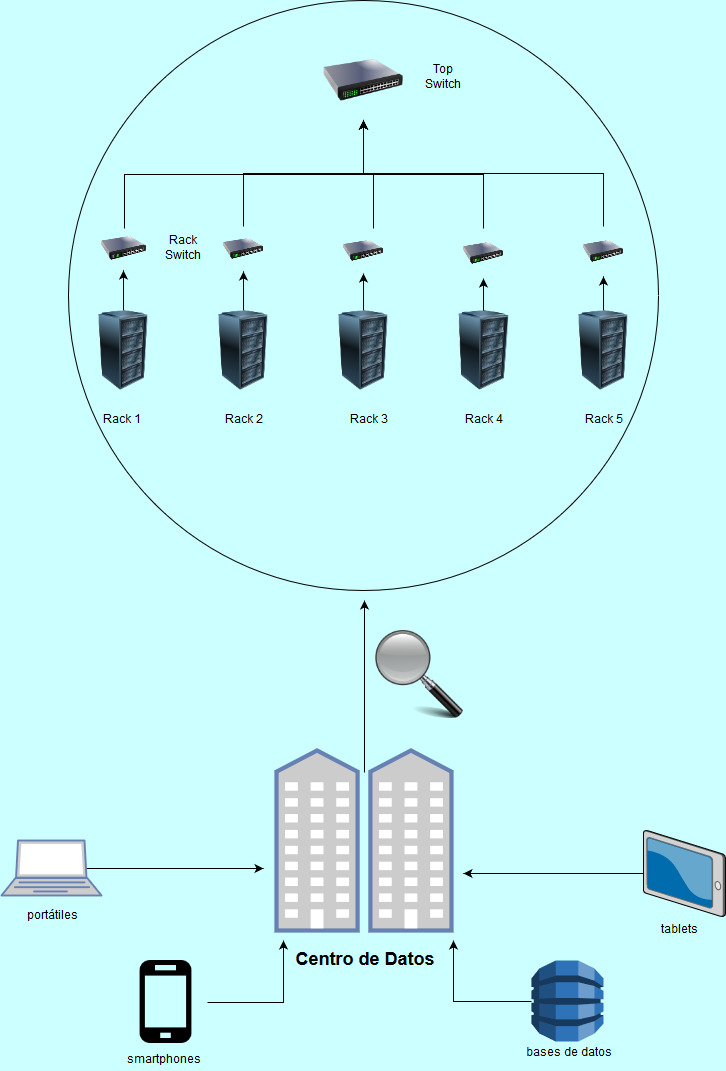
\includegraphics[scale=0.5]{C:/Users/David/Desktop/TFG/TFGLatex/imagenes/cluster_topology.jpg}
  \caption[Topología de un \textit{cluster}]{Topología de un \textit{cluster}}
  \label{cluster_topology}
\end{figure}

\clearpage


\section{Topología de un \textit{cluster Hadoop}}
Como se ha mencionado en la \autoref{sec:que_es_apache_hadoop}, \textit{Hadoop} este se compone de dos partes 
fundamentales. Cada una de esas partes se compone de subprocesos que se encargan de distintas tareas por lo que
lo primero que debemos hacer es elegir máquinas con una configuración de \textit{hardware} 
adecuada a los servicios que se va a desplegar en ella.

En \textit{clusters} destinados a producción, la mejor opción es utilizar \textit{Cloudera Manager} para
su despliegue. El asistente gráfico y todos los servicios que lleva por detrás irán instalados en una
sola máquina. \\
El resto de servicios propios de \textit{Hadoop} pueden ser instalados en una sola máquina (esto se conoce 
como modo pseudodistribuido\index{Pseudodistribuido}) o en varias máquinas (modo distribuido).
Como regla general, se necesitan mínimo dos máquinas \textit{master}, tres máquinas \textit{worker} y una
máquina \textit{gateway} para tener un \textit{cluster} plenamente funcional.
\newline

Respecto a los servicios de \textit{HDFS} y \textit{YARN} hay que tener ciertas consideraciones,
por ejemplo, la máquina designada como \textit{NameNode} necesitará mas memoria \textit{RAM} 
debido a que este guarda toda la información de los metadatos de los archivos en memoria. 
También, las máquinas que designemos como trabajadoras será recomendable que tengan buenos recursos 
de \textit{CPU} y memoria así como conexión de red de alta velocidad, de esta manera los trabajos 
que subamos al \textit{cluster} se ejecutaran de manera mas rápida.
Las máquinas \textit{worker} será muy recomendable que lleven instalados los servicios de 
\textit{NodeManager} y \textit{DataNode} conjuntamente, si bien no es obligatorio.
Para un conocimiento mas profundo acerca de los servicos de \textit{Hadoop}, ver 
\url{http://hadoop.apache.org/docs/current/}
\newline

A continuación, se muestra un esquema de un \textit{cluster Hadoop} con una configuración básica de los dos 
servicios mencionados anteriormente.

\begin{figure}[h]
  \centering
  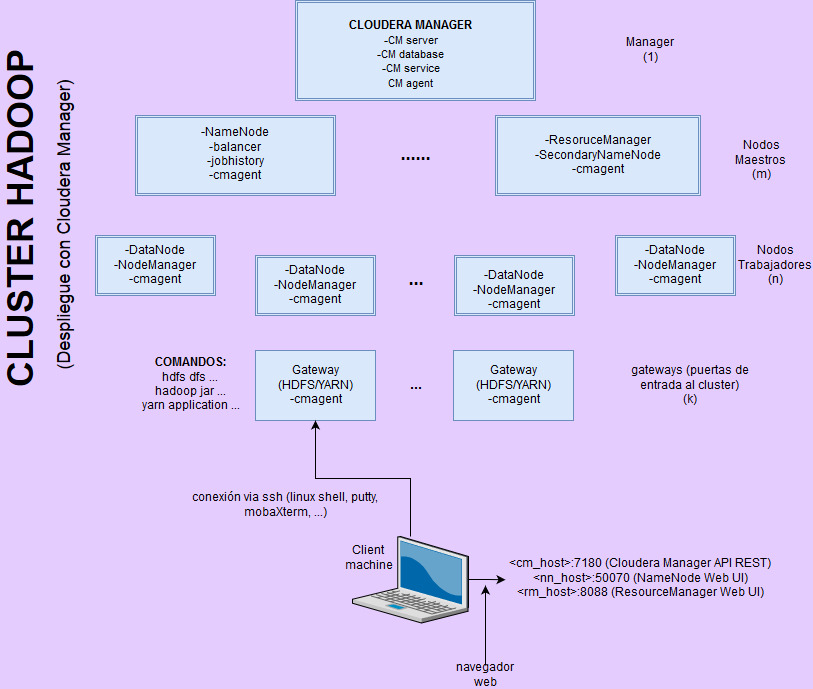
\includegraphics[scale=0.5]{C:/Users/David/Desktop/TFG/TFGLatex/imagenes/hadoop_topology.jpg}
  \caption[Servicios de un \textit{cluster Hadoop}]{Servicios de un \textit{cluster Hadoop}}
  \label{hadoop_topology}
\end{figure}

\clearpage